\setcounter{chapter}{7-1}

\chapter{Neural Networks 2 - Training Techniques, Regularization}

\setcounter{section}{6}

\section{Optimizing neural network parameters}

    We now understand both how neural networks work, and how to \textbf{train} them. We can use gradient descent to \textbf{optimize} their parameters.
    
    But, we can do \textbf{better} than a simple SGD approach with step size $\eta(t)$. We'll try out some \textbf{modifications} that can speed up our training, and make better models.

    \pagebreak
    \subsection{Mini-batch}
    
        \subsubsection{Review: Gradient Descent Notation}
        
            Let's review some gradient descent notation. We want to \textbf{optimize} our objective function $J$ using $W$.
            
            We do this using the gradient. This gradient depends on our current weights at time $t$, $\blu{W_{t}}$.
            
            \begin{equation}
                \overbrace{
                    \;\;
                    \nabla_W J
                    \;\;
                }^{\text{General Gradient}}
                \quad
                \longrightarrow
                \quad
                \overbrace{
                    \nabla_W J ( \blu{ W_{t} } )
                }^{\text{Gradient at time $t$}}
            \end{equation}
            
            Our update rule is:
            
            \begin{equation}
                \red{ W_{\text{new}} }
                \;\;=\;\;
                \blu{ W_{\text{old}} }
                \;\;-\;\;
                \eta
                \overbrace{
                    \Big(
                        \nabla_W J ( \blu{ W_{\text{old}} } )
                    \Big)
                }^{\text{Gradient}} 
            \end{equation}
            
            Or, using timestep $t$:
            
            \begin{equation}
                \red{ W_{t+1} } 
                \;\;=\;\;
                \blu{ W_t }
                \;\;-\;\;
                \eta
                \overbrace{
                    \Big(
                        \nabla_W J ( \blu{ W_t } )
                    \Big)
                }^{\text{Gradient}}
            \end{equation}
            
            What is our objective function $J$? Without regularization, it's based on our \textbf{loss} function. We can get loss for each of our data points:
                \note{We won't define $J$ here, because it is slightly different for SGD and BGD. We'll get to that below.}
            
            \begin{equation}
                \ex{\loss}{i}
                =
                \overbrace{
                    \loss(
                    \; \ex{g}{i} \;
                    ,\eyi
                    )
                }^{\text{Loss for data point $i$}}
            \end{equation}
            
            Our guess $\ex{g}{i}$ depends on both our current data point $\exi$, and the current weights $\blu{ W_t }$:
            
            \begin{equation}
                \ex{\loss}{i}(\blu{ W_t })
                \;\;=\;\;
                \loss(
                \;\;
                \overbrace{
                     h(\exi;\blu{ W_t }) 
                }^{\ex{g}{i}}
                \;\;
                ,\eyi
                )
            \end{equation}
    
        \phantom{}
    
        \subsubsection{Review: BGD vs. SGD}
        
            Let's review our two main types of gradient descent, using the equation
            
            \begin{equation}
                \red{ W_{t+1} } 
                \;\;=\;\;
                \blu{ W_t }
                \;\;-\;\;
                \eta
                \overbrace{
                    \Big(
                        \nabla_W J ( \blu{ W_t } )
                    \Big)
                }^{\text{Gradient}}
            \end{equation}
            
            First, we have \textbf{batch gradient descent}, where we use our \textbf{whole} training set each time we take a step.\\
            
            \begin{definition}
                \vocab{Batch Gradient Descent (BGD)} is a form of gradient descent where we get the \gren{gradient} of our loss function using \purp{all of our training data}.
                
                \begin{equation*}
                    \nabla_W J ( \blu{ W_t } )
                    \;\;=\;\;
                    \sum_{i=1}^n
                    \;\;
                    \overbrace{
                        \nabla_W
                        \Big(
                            \ex{\loss}{i}(\blu{ W_t })
                        \Big)
                    }^{\text{Each data point}}
                \end{equation*}
                
                We get the gradient for each data point, and then \purp{add} all of those gradients up. We use this \purp{combined gradient} to take \gren{one step}.
                
                We \gren{repeat} this process every time we want to take a new step.
            \end{definition}
            
            Then, we have \textbf{stochastic gradient descent}, where we use only \textbf{one} data point for each step we take.\\
            
            \begin{definition}
                \vocab{Stochastic Gradient Descent (SGD)} is a form of gradient descent where we get the \gren{gradient} of our loss function using \purp{one data point at a time}.
                
                \begin{equation*}
                    \nabla_W J ( \blu{ W_t } )
                    \;\;
                    =
                    \;\;
                    \overbrace{
                    \nabla_W
                    \Big(
                        \ex{\loss}{i}(\blu{ W_t })
                    \Big)
                    }^{\text{One data point}}
                \end{equation*}
                
                We \purp{randomly} choose one data point $(\exi,\eyi)$ and get the \purp{gradient}. Based on this one gradient, we take our \gren{step}.
                
                For each step, we choose a new \purp{random} data point.
            \end{definition}
            
            These two approaches have tradeoffs:\\
            
            \begin{concept}
                There are \vocab{tradeoffs} between \vocab{SGD} and \vocab{BGD}:
                
                \begin{itemize}
                    \item Each step is \purp{faster} in \purp{SGD}: we only use one data point. 
                        \begin{itemize}
                            \item Meanwhile, \gren{BGD} is \gren{slower}: each step uses all of our data.
                            \item \purp{SGD} could improve a lot with only a \orgg{small subset} of a data.
                        \end{itemize}

                        \phantom{}
                        
                    \item Because \gren{BGD} uses all our data, its gradient is much more \gren{accurate}.
                        \begin{itemize}
                            \item \purp{SGD} often uses \purp{smaller} steps: the gradient is less accurate, with less data.
                            \item This is worse if the data is \orgg{noisy}: each SGD step becomes less effective.
                        \end{itemize}

                        \phantom{}
                        
                    \item \purp{SGD} \purp{randomly} chooses data points: this random noise makes it harder to overfit.
                        \begin{itemize}
                            \item \gren{BGD} uses all of the data, so we don't reduce overfitting.
                        \end{itemize}
                \end{itemize}
            \end{concept}
        
        \phantom{}
        
        \subsubsection{Mini-batch}
        
            Rather than picking one or the other, one might think, "why do we have to pick \textbf{every} data point or \textbf{one} data point? Couldn't we pick only a \orgg{few}?"
            
            This is the premise of \textbf{mini-batch}: instead of making a batch out of the entire training set, we \textbf{randomly} select a few data points, and use that as our batch.\\
            
            \begin{definition}
                \vocab{Mini-batch} is a way to \purp{compromise} between SGD and BGD.
                
                To create a mini-batch, we \purp{randomly} select $K$ data points from our training data. 
                
                We treat this mini-batch the same way we would a regular \gren{batch}: get the \purp{gradient} of each data point, \gren{add} those gradients, and take one  step of gradient descent.
                
                \begin{equation*}
                    \nabla_W J ( \blu{ W_t } )
                    =
                    \overbrace{
                        \sum_{i=1}^K
                    }^{K \text{ data points in a mini-batch}} 
                    \nabla_W
                    \Big(
                        \ex{\loss}{i}(\blu{ W_t })
                    \Big)
                \end{equation*}
                
                We gather a \gren{new} mini-batch for each step we want to take.
            \end{definition}
            
            Mini-batch is the \textbf{default} used in most modern packages: it gives us more \textbf{control} over our algorithm, and can often find the \textbf{best} of both worlds.
                \note{We do have to be careful to randomly select data in an efficient way, though. Packages usually take care of this.}\\
            
            \begin{concept}
                \vocab{Mini-batch} has a lot of benefits of both SGD and BGD:
                
                \begin{itemize}
                    \item Steps are \purp{faster} than BGD: we only need to get the gradient for $K$ points.
                        \begin{itemize}
                            \item The \orgg{speed} no longer depends on the total training data size (more data, more gradients): instead, it depends on our \orgg{batch size} $K$.
                        \end{itemize}
                        
                    \item Steps are more \purp{accurate} than SGD: with more data, we have a better \gren{gradient}.
                        \begin{itemize}
                            \item This means we can take \purp{bigger} steps.
                        \end{itemize}
                    
                    \item Our batches are \purp{random}, like SGD: we reduce overfitting and escape local minima.
                \end{itemize}

                \phantom{}
                
                One more important benefit:
                
                \begin{itemize}
                    \item If we find that a particular problem is better suited for something closer to BGD or SGD, we can \gren{adjust} our batch size $K$.
                        \begin{itemize}
                            \item This gives us more \purp{control} over our learning algorithm.
                        \end{itemize}
                \end{itemize}
            \end{concept}
        
    \phantom{}
    \pagebreak
    \subsection{Adaptive Step Size - Challenges}
    
        We'll stop discussing mini-batches, and the SGD vs. BGD problem. Instead, let's improve our \gren{step size}.
        
        Step size $\eta$ is a difficult problem:
        
        \begin{itemize}
            \item If $\eta$ is \purp{small}, then our training can take a long \textbf{time}.
            
            \item If $\eta$ is too \purp{large}, we might \textbf{diverge}: our answer gets way too large.
            
            \item A \textbf{large} step size might also cause \orgg{oscillation}: most of our step is wasted going back and forth, so we go \textbf{slowly} again.
        \end{itemize}
        
        SGD and mini-batch have a step size-related problem, too:
        
        \begin{itemize}
            \item In order to \textbf{converge} according to our theorems (see chapter 3), the step size $\eta(t)$ has to be \textbf{decreasing} in a certain way.
                \note{Check chapter 3 for the exact requirements of the theorem.}
        \end{itemize}

        In Appendix B, we discuss some common techniques:

        \begin{itemize}
            \item Momentum
            \item Adadelta
            \item Adam
        \end{itemize}
    
    \phantom{}

    
    \pagebreak
    \subsection{Vanishing/Exploding Gradient}
    
        Now, neural networks have one more \textbf{problem}, that we've ignored so far: \textbf{deep} neural networks can cause a problem called "\vocab{exploding/vanishing gradient}".
            \note{By "deep", we just mean "many layers".}
        
        Here's an example: suppose you have a long chain rule, with 8 terms. Our chain rule gets \textbf{longer} with more layers, because each layer needs its own derivatives.
        
        \begin{equation}
            \pderiv{A}{H}
            \;\;=\;\;
            \pderiv{A}{B}
            \cdot
            \pderiv{B}{C}
            \cdot
            \Big(
            \cdots
            \Big)
            \cdot
            \pderiv{G}{H}
        \end{equation}
        
        This chain rule gets \textbf{longer} as we move "\textbf{backwards}" through our network, so the chain rule is longest for the "\textbf{early}" layers: $\ell=1, 2,$ and so on.
        
        Suppose all of our derivatives are roughly $.1$. What happens when we multiply them \textbf{together}?
        
        \begin{equation}
            \pderiv{A}{H}
            \;\; = \;\;
            .1 \cdot .1 \cdot 
            \Big(
            \cdots
            \Big)
            \cdot 
            .1
            \;\; = \;\;
            10^{-8}
        \end{equation}
        
        The derivative becomes really, really \gren{tiny}! This is the case of the \textbf{vanishing} gradient: if our gradients are less than one, then as we append more layers, they multiply to get smaller and smaller.

        \begin{itemize}
            \item This is a problem: if our gradients in our earlier layers become too \textbf{small}, we'll never make any progress! They'll hardly change.\\
        \end{itemize}
        
        
        
        \begin{definition}
            \vocab{Vanishing gradient} occurs when a deep neural network ends up with \purp{very small gradients} in the \gren{earlier} layers. 
            
            This happens because a deeper neural network has a \gren{longer chain rule}: if all of the terms are \purp{less than one}, they'll multiply into a very small value, "\vocab{vanishing}".
            
            This means that our gradient descent will have \purp{almost no effect} on these earlier weights, \gren{slowing down} our algorithm considerably.
        \end{definition}
        
        What if the gradients are larger than 1? Let's say our derivatives are 10 each.
        
        \begin{equation}
            \pderiv{A}{H}
            = 
            10 \cdot 10 \cdot 
            \Big(
            \cdots
            \Big)
            \cdot 
            10
            =
            10^{8}
        \end{equation}
        
        Now, the early derivatives are becoming \textbf{huge}! This is the case of \textbf{exploding} gradient: if our gradients are greater than one, then as we add layers, they multiply to get bigger.

        \begin{itemize}
            \item This is also a problem: we don't want to take \textbf{huge} steps, or we will \textbf{diverge}, or \textbf{oscillate}, and jump huge distances across the \textbf{hypothesis space}.\\
        \end{itemize}
        
        
        
        \begin{definition}
            \vocab{Exploding gradient} occur when a deep neural network ends up with \purp{very large gradients} in the \gren{earlier} layers. 
            
            This happens because a deeper neural network has a \gren{longer chain rule}: if all of the terms are much \purp{greater than one}, they'll multiply into a very large value, "\vocab{exploding}".
            
            This means that our gradient descent will take \purp{huge steps} in the hypothesis space. This can cause us to \gren{diverge}, miss local minima, or \gren{oscillate}.
        \end{definition}
        
        So, to avoid this, we can't just blindly multiply our gradients and keep a fixed step size.
        
        The solution? Each \textbf{weight} gets its own step size $\eta$.\\
        
        \begin{concept}
            In order to avoid \vocab{vanishing/exploding} gradient problems, we give each \gren{weight} in our network its own \purp{step size} $\eta$.
            
            This allows us to \purp{adjust} the step size for some weights more than others: if our gradient is too large or small, we can fix it.
        \end{concept}


    \pagebreak
    
    
        
            




\pagebreak

\section{Regularization}

    Something we haven't discussed in a while, that we might investigate, is \orgg{regularization}: techniques against overfitting.

    \begin{itemize}
        \item We teach our model using "training data", which, by chance, may not perfectly reflect the \textbf{true} distribution.
    \end{itemize}

    We want to apply this to our modern, deep neural networks, with their huge number of \textbf{parameters}, and huge amount of \textbf{data}. And yet...
    
    These modern neural nets \gren{don't} tend to have as much problem with \purp{overfitting}, and we're not sure \textbf{why}!

    Regardless, we do still have \textit{some} methods for regularization: this will be our focus for the rest of this chapter.

    \subsection{Methods related to ridge regression}

        We'll start with methods that we can bring back from classic ridge regression.

        \subsubsection{Early Stopping}

            One component built into our learning algorithm for regression is \purp{early stopping}: we check if the model is still making \textbf{progress}. If it isn't, then we \textbf{stop} training.

            \begin{itemize}
                \item The longer we train our model, the more time it has to "\textbf{memorize}" the exact structure of our training data: including \textbf{noise}.
            \end{itemize}

            We would typically either measure the size of the \gren{gradient}, or the change in the \purp{loss}. If either was small, then we might be in a local minimum: we've finished training.

            \phantom{}

            So, we do the same here: after a period of training (over the whole dataset, called an \vocab{epoch}), we measure the \textbf{loss} on a validation set.

            \begin{itemize}
                \item If the loss stops decreasing, or begins \orgg{increasing}, our model is probably \textbf{overfitting}. We \redd{stop early}.
            \end{itemize}

            Then, you return the weights with the lowest error.\\

            \begin{definition}
                An \vocab{epoch} is the time frame during which your model sees your whole \purp{training data} set, \orgg{once}.

                \begin{itemize}
                    \item Note that sometimes, "epoch" just refers to how long you train before you check your loss.
                    \item In this case, it might be smaller than the whole dataset.
                \end{itemize}
            \end{definition}

            \phantom{}

            \begin{definition}
                With \vocab{early stopping}, you evaluate your model using your \purp{validation data}, computing the loss.

                \begin{itemize}
                    \item If the loss has decreased from the last epoch, you \gren{continue} training.
                    \item If the loss has stopped decreasing, or is increasing, you \redd{stop} training.
                \end{itemize}

                This continues until you've either run out of \textbf{epochs}, or you've met your \textbf{termination} condition, and stopped early.
            \end{definition}


            \subsubsection{Weight Decay}

                We can also use the same kind of regularization term that we used for linear regression: penalizing the \purp{squared magnitude}.

                \begin{itemize}
                    \item Starting with our loss function:
                        \begin{equation}
                            J_{loss} = \sum_{i = 1}^{n}
                                \mathcal{L}( \red{\text{NN}(x^{(i)})},\;\; \blu{y^{(i)}};\;\; \grn{W})
                        \end{equation}
                    \item And we penalize based on the square magnitude of our weights:
                        \begin{equation}
                            J = \lambda \norm{\grn{W}}^2 +
                                J_{loss}
                        \end{equation}
                \end{itemize}

            If we take the gradient, we get:

            \begin{equation}
                \nabla_W J = 2\lambda \grn{W} + 
                    \nabla_W J_{loss}
            \end{equation}

            Let's see how the regularization affects our step:

            \begin{equation}
                \grn{W_t} = 
                \grn{W_{t-1}} - 
                \eta \Big( 2\lambda \norm{\grn{W_{t-1}}} + 
                     \nabla_W J_{loss} \Big)
            \end{equation}

            It directly subtracts from our weight, \orgg{decaying} it.

            \begin{equation}
                \grn{W_t} = 
                \grn{W_{t-1}} \Big( \org{ 1 -  2\lambda \eta } \Big)  - 
                     \eta \nabla_W J_{loss} 
            \end{equation}

            Thus, we call it \textbf{weight decay}.\\

            \begin{concept}
                When we apply \purp{square magnitude} regularization to the weights of a neural network, we call it \vocab{weight decay}.

                \begin{equation*}
                    J_{reg} = J_{loss} + \lambda \norm{W}^2
                \end{equation*}

                That's because, when you take the gradient, it directly subtracts from weight $W$, causing it to \orgg{decay} by a factor of $(1-2\lambda \eta)$.

                \begin{equation*}
                    \grn{W_t} = 
                    \grn{W_{t-1}} \Big( \org{ 1 -  2\lambda \eta } \Big)  - 
                         \eta \nabla_W J_{loss} 
                \end{equation*}
            \end{concept}

        \subsubsection{Perturbation}

            One last way to reduce overfitting is to add some \orgg{random noise} to our data: each variable has a small, random number added to it.

            This value is typically \purp{zero-mean} and \gren{normally distributed}:

            \begin{itemize}
                \item Zero-mean: it has 0 effect, on average, so it doesn't bias the data high or low.
                \item Normally distributed: the noise is \textbf{symmetric}: +2 and -2 are equally likely.
                    \note{The "normal distribution" contains more information than that, but the symmetry is important.}
            \end{itemize}

            How large the noise is, depends on the chosen \textbf{variance}.
            
            This reduces overfitting, because if the data is slightly different each time you see it, it's harder to perfectly "memorize" the exact shape and structure.\\

            \begin{definition}
                \vocab{Perturbation} is a technique where you slightly modify your system.

                \begin{itemize}
                    \item In our case, we're \gren{randomly} adding small amount of \purp{noise} to our input data.
                \end{itemize}

                This makes it more difficult for the model to \orgg{overfit}, because the patterns aren't always exactly the same.

                \begin{itemize}
                    \item Only the "general", high-level patterns are preserved, each time you view the dataset.
                \end{itemize}
            \end{definition}

            Of course, if you perturb your data too strongly, you can miss real patterns. Your perturbations shouldn't be too large.

            

    \subsection{Dropout}

        We also have \textbf{structural} ways of dealing with overfitting. We discussed perturbing the \purp{dataset}, but we could, instead, perturb the \gren{model} itself!

        

        We do this by randomly \redd{removing} some weights from the neural network, and training. 

        \begin{itemize}
            \item Each weight has a probability $p$ of being "turned off": the \textbf{activation} is set to zero.

            \begin{equation}
                a^\ell_j=0
            \end{equation}

            \item Thus, that neuron's output is \textbf{ignored} by the next layer, and receives no training.

            \item At the next step, we remove a \textbf{different} random selection of weights. 
        \end{itemize}

        Because our model keeps changing slightly, it's harder to exactly \textbf{overfit} to the data.

        \phantom{}

        This particular approach also addresses a \textbf{different} kind of overfitting:

        \begin{itemize}
            \item One model might heavily "rely" on a \textbf{small} number of neurons to make decisions.
            \item This makes our model less flexible, uses the weights less efficiently.
        \end{itemize}
        
        To solve this, we prevent the neural network from using some of these weights, \textbf{randomly}.

        Thus, the whole network "\textbf{shares}" some responsibility for  getting the right answer.\\

        \begin{definition}
            \vocab{Dropout} is a process where, at each training interval, you \orgg{randomly} "drop out", or de-activate, some of the weights in the network.

            \begin{itemize}
                \item Each neuron has probability $p$ of being turned off.
                \item These neurons have their \gren{activation} set to zero: $a^\ell_j=0$.
            \end{itemize}

            This process is designed to reduce \purp{overfitting}. As the network randomly changes, it's harder for it to perfectly match the data structure.

            This process is also designed to create "collective responsibility" for your neurons. It prevents your network from relying on a small number of neurons to solve problems.

            It generally improves \orgg{robustness} against random variations in the data.
        \end{definition}

        \phantom{}

        \begin{clarification}
            When a network using dropout is finished training, we multiply all the weights by $p$. Why?

            \begin{itemize}
                \item Because during training, only $p$ fraction of the neurons were active. 
                \item We want to replicate that average activity level, even when we use all of our neurons.
            \end{itemize}
        \end{clarification}

        

        \phantom{}

        This approach has, in recent years, become somewhat less popular, for a couple reasons:

        \begin{itemize}
            \item Very \textbf{large} networks don't struggle as much with overfitting.
            
            \item CNNs tend not to benefit from this procedure, because of \textbf{weight-sharing}: the same weights are re-used in multiple places.
                \note{We'll discuss CNNs in our next chapter.}

            \item Like most ML techniques, their usefulness depends on the situation.
        \end{itemize}

        It still finds use in some smaller models, RNNs, etc.

        In many places, it has been replaced by \vocab{batch normalization}.

    \pagebreak

    \subsection{Batch Normalization}

        \subsubsection{Covariate Shift}

            Our last approach related to regularization was designed to handle a new type of problem we call \textbf{covariate shift}:
            
            When you run \textbf{gradient descent} on a neural network, you're adjusting the weights of all of our layers, at the \textbf{same time}.
    
            Let's focus on layer 1 and layer 2. By updating layer 1, we've changed the outputs it creates: the same $\ex{x}{i}$ now creates a different output, going from $a^1_{old}$ to $a^1_{new}$.
    
            But, this output is the \textbf{input} of layer 2.
            
            \begin{itemize}
                \item This means that layer 2 is now receiving \purp{different inputs} than it was before.
                    
                \item This is a problem: layer 2 just received training based on the \gren{old} inputs $a^1_{old}$!
            \end{itemize}
    
            This makes life a lot harder for our layer 2: not only is it learning to make better predictions, it also has to adjust for the change in layer 1. This is a form of \vocab{covariate shift}.\\
    
            \begin{definition}
                \vocab{Covariate shift} occurs when the distribution of input variables \purp{changes} over time. 
    
                \begin{itemize}
                    \item This can cause our original model to become inaccurate, or "outdated": it was trained on \purp{different} data.
                \end{itemize}
    
                \vocab{Internal covariate shift} occurs because of changes to the network itself.
                
                \begin{itemize}
                    \item The distribution of inputs to \gren{later layers} changes, because \gren{earlier layers} have changed through training.
                \end{itemize}
            \end{definition}
    
            \miniex If the weights in layer 1 all get smaller (as a side effect of correcting them), layer 2 may have to make all of its weights bigger to compensate.
            
            \begin{itemize}
                \item Our expectation is that this extra work would slow down training.
            \end{itemize}

        \subsubsection{Layer Normalization}

            So, we want to counter the problem of how the input to layer 2 \textbf{changes} based on layer 1's \textbf{learning}.

            \begin{itemize}
                \item But, at the same time, we don't want to \textbf{undo} the work that we did \textbf{training} layer 1.
                \item So, we want to preserve the information in layer 1, while making it easier to use.
            \end{itemize}

            In our example, we mentioned that the scale of the inputs might get larger: they all get bigger or smaller, at the same time.

            But, we often want to know what makes these inputs \textbf{different} from each other, so we can compare them: it's not helpful if all of them become larger/smaller.

            So, we'll \vocab{standardize} each of our mini-batches of data, between each layer:
                \note{This is exactly the same as when we standardized in the Feature Transformation chapter.}

            \begin{itemize}
                \item \purp{Subtracting the mean}: we take the mean of the mini-batch input, and subtract it from each data point. So, our standardized data is always centered at 0.

                \item \gren{Dividing by standard deviation}: we compute how "spread out" the data is, and scale by that factor. Our standardized data is always the same amount "spread out".
            \end{itemize}

            We repeat this process in between each layer of our network. Each layer receives a set of inputs with mean 0, standard deviation 1, no matter how the earlier layers change.
                \note{Below, we exclude the $\ell$ superscript in $z^\ell$, $\mu^\ell$, $\sigma^\ell$, and $n^\ell$ for readability.}

            For now, we'll apply this to the pre-activation $Z$.\\

            \begin{notation}
                We'll represent the element in the $\nth{i}$ row, $\nth{j}$ column, as $Z_{ij}.$
            \end{notation}

            \phantom{}

            \begin{kequation}
                *Here, we focus on a single element: dimension $i$ of the $\nth{j}$ data point in our batch, $z_{ij}$.
            
                When we \vocab{standardize}, we first compute the \gren{mean} and \purp{standard deviation}:

                \begin{equation*}
                        \blu{\mu_i} =\frac{1}{K} \sum_{j=1}^K \red{Z_{ij}}
                        \qquad
                        \sigma^2_i = \frac{1}{K} \sum_{j=1}^K (\red{Z_{ij}}-\blu{\mu_i})^2 
                    \end{equation*}

                Once we've done that, we can properly standardize, creating data with mean 0, and sd 1.

                \begin{itemize}
                    \item We include a very small $\epsilon$ term to avoid dividing by zero.
                \end{itemize}

                \begin{equation*}
                        \red{ \overline{Z}_{ij} } =  \frac{ \red{Z_{ij}}  -\blu{\mu_i}}{\sigma_i+\epsilon}
                    \end{equation*}
                
            \end{kequation}

            \begin{concept}
                In order to deal with \vocab{internal covariate shift}, we'll take each mini-batch of $k$ \gren{pre-activations} to each \gren{layer} of our neural network, and \purp{standardize}/normalize it.

                \begin{itemize}
                    \item Each \orgg{dimension} of the input is standardized \orgg{separately}.
                \end{itemize}

                After \purp{standardizing}, this data is sent forward through the network.

                \begin{itemize}
                    \item This is equivalent to using a "standardizing function" \orgg{after} the weight function $Z=W^TA$, and \orgg{before} the activation function $f(Z)$ (now $f(\overline{Z})$).
                    \item We could also standardize \textbf{after} activation, but it's unclear which approach is better.
                \end{itemize}
                
            \end{concept}

            We can insert our new module into our existing model:


            \begin{figure}[H]
                \centering
                    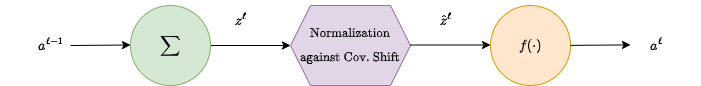
\includegraphics[width=100mm,scale=0.5]{images/nn_2_images/cov_shift_neuron.png}
                
                \caption*{Normalization/standardization can be treated just like any other module.}
            \end{figure}

            \phantom{}

            Note that this preserves the \orgg{information} in our input data:
            
            \begin{itemize}
                \item If one data point has one feature much larger than another, you'll still see that: the gap will just be shifted over to zero, and normalized.
                
            \end{itemize}

            \miniex Suppose you have some data: $[1,2,\red{100},3,4,5]$. If you standardize, you get

            \begin{equation}
                [-0.458, -0.433, \red{2.04}, -0.408, -0.383, -0.358, ]
            \end{equation}

            The larger data point still stands out above the rest!
            
            We need to be careful of dimensions:\\

            \begin{clarification}
                Normalization relies on the distribution (mean, s.d.) of our \purp{mini-batch}.

                But that means we can't just compute one data point at a time: we need to include the whole mini-batch of $k$ \gren{at the same time}.

                So, we have to change the dimensions of $Z^\ell$.

                $k$ is our \purp{batch size}, while $n$ is the number of \gren{dimensions}. 
                

                \begin{itemize}
                    \item $Z^\ell$ without norm: $(n^\ell \times 1)$
                    \item $Z^\ell$ with norm: $(n^\ell \times \red{k})$
                \end{itemize}

                We use $Z_{ij}^\ell$ to indicate the $\nth{i}$ dimension of the $\nth{j}$ data point.
            \end{clarification}
            

        

        \subsubsection{Post-Normalization: Choose Mean and S.D.}

            Now, we've adjusted it so that our distribution doesn't "drift", based on our training.

            But, now, we've \textbf{restricted} our model:
            
            \begin{itemize}
                \item We don't necessarily want our mean and standard deviation to be 0 and 1: it would be better to be able to \textbf{control} it.
            \end{itemize}
            
            To accomplish this, we'll \textbf{scale} and \textbf{shift} our input. Thus, we're choosing our mean/s.d. in a deliberate way.
            
            \begin{itemize}
                \item Each dimension needs its own mean and standard deviation.
                \item We have $n$ dimensions, and we need one variable to handle mean (or s.d.) for each: we'll need an $(n \times 1)$ vector.\\
            \end{itemize}

            \begin{concept}
                By doing \orgg{normalization}, we've transformed $Z$ into $\overline{Z}$. 
                
                \begin{itemize}
                    \item This "resets" our mean and standard deviation to 0 and 1.
                \end{itemize}

                However, we want to be able to \textbf{control} our mean and standard deviation. To do so, we introduce two new parameters:

                \begin{itemize}
                    \item $G$: An $(n \times 1)$ vector that \purp{scales} each of our dimensions $\overline{Z}_i$, giving our \purp{standard deviations}.
                    \item $B$: An $(n \times 1)$ vector that \gren{shifts} each of our dimensions $\overline{Z}_i$, giving our \gren{means}.
                \end{itemize}

                Thus, we get the true output of \vocab{batch normalization}:

                \begin{equation*}
                    \red{\widehat{Z}_{ik}} = \pur{G_i} * \red{\overline{Z}_{ij}} + \grn{B_i}
                \end{equation*}

            \end{concept}

            \miniex Here's a sample example using a vector $\overline{z}_j$: only considering one, post-normalization data point $j$. 

            \begin{equation}
                \begin{bmatrix}
                    \widehat{Z}_{1j} \\  \widehat{Z}_{2j} \\ \vdots \\ \widehat{Z}_{kj}
                \end{bmatrix}
                =
                \begin{bmatrix}
                    G_{1} \\  G_{2} \\ \vdots \\ G_{k}
                \end{bmatrix}
                *
                \begin{bmatrix}
                    \overline{Z}_{1j} \\  \overline{Z}_{2j} \\ \vdots \\ \overline{Z}_{kj}
                \end{bmatrix}
                +
                \begin{bmatrix}
                    B_{1} \\  B_{2} \\ \vdots \\ B_{k}
                \end{bmatrix}
            \end{equation}

            Where $*$ indicates element-wise multiplication.

            If we include this in our neuron graph, we now have two new modules:

            \begin{figure}[H]
                \centering
                    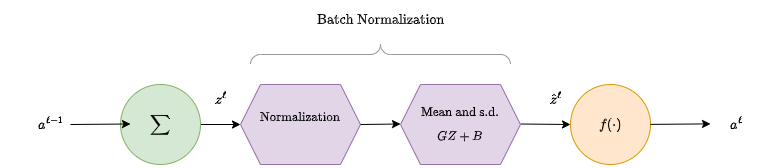
\includegraphics[width=120mm,scale=0.5]{images/nn_2_images/batch_normalization.png}
            \end{figure}

            \subsubsection{Full definition}


            \begin{definition}
                \vocab{Batch Normalization} is a process where we

                \begin{itemize}
                    \item Standardize the pre-activation for each layer using the mean $\mu_i$ and standard deviation $\sigma_i$ (for the $\nth{i}$ dimension). Select $\epsilon$: $0 < \epsilon<<1$.

                    \begin{equation*}
                        \red{ \overline{Z}_{ij} } =  \frac{ \red{Z_{ij}}  -\blu{\mu_i}}{\sigma_i+\epsilon}
                    \end{equation*}
                    
                    \item Choose the new mean and standard deviation for the pre-activation using $(n \times 1)$ vectors $G$ and $B$

                    \begin{equation*}
                        \red{\widehat{Z}_{ik}} = \pur{G_i} * \red{\overline{Z}_{ij}} + \grn{B_i}
                    \end{equation*}
                \end{itemize}
                
            \end{definition}

            \phantom{}

            \begin{concept}
                \vocab{Batch Normalization} is meant to accomplish the following:

                \begin{itemize}
                    \item Remove possible \purp{internal covariance shift}: training earlier layers may change the scale of inputs to later layers.
                        \begin{itemize}
                            \item This could make training more difficult.
                        \end{itemize}
                    \item Allow our model to \gren{select} a particular mean and s.d. for its pre-activation values, rather than arriving at them by chance.
                \end{itemize}

                It also tends to have a regularizing effect, and, in some learning algorithms, has replaced dropout.
            \end{concept}

        \subsubsection{Effectively Perturbs Data}

            We're not actually sure why normalization helps our models train. We originally designed it for \textbf{internal covariate shift}, but we're not sure if that's really \textbf{why} it works.

            One explanation might be that, due to random sampling, each mini-batch ends up slightly \textbf{modified} by our normalization.
            
            \begin{itemize}
                \item Since each batch is likely to have a slightly different mean/standard deviation, each one ends up differently "perturbed" by normalization.
            \end{itemize}

        \subsubsection{Applying batch normalization to backprop}

            We defer discussion of backprop to Appendix B.

    \pagebreak


\pagebreak
\section{Terms}
    \subsection*{Section 7-1}

    \begin{itemize}
        \item Neuron (Unit, Node)
        \item Neural Network
        \item Series and Parallel
        \item Linear Component
        \item Weight $w$
        \item Offset (Bias, Threshold) $w_0$
        \item Activation Function $f$
        \item Pre-activation $z$
        \item Activation $a$
        \item Identity Function
        \item Acyclic Networks
        \item Feed-forward Networks
        \item Layer
        \item Fully Connected
        \item Input dimension $m$
        \item Output dimension $n$
        \item Weight Matrix
        \item Offset Matrix
        \item Layer Notation $A^\ell$
        \item Step function
        \item ReLU function
        \item Sigmoid function
        \item Hyperbolic tangent function
        \item Softmax function
    \end{itemize}

    \subsection*{Section 7-1.5}

    
    \begin{itemize}
        \item Forward pass
        \item Back-Propagation
        \item Weight gradient
        \item Matrix Derivative
        \item Partial Derivative
        \item Multivariable Chain Rule
        \item Total Derivative
        \item Size of a matrix
        \item Planar Approximation
        \item Scalar/scalar derivative
        \item Vector/scalar derivative
        \item Scalar/vector derivative
        \item Vector/vector derivative
        
    \end{itemize}

    \subsection*{Section 7-2}

    \begin{itemize}
        \item Mini-batch
        \item Vanishing/Exploding Gradient
        \item Momentum (Optional)
        \item Adadelta (Optional)
        \item Adagrad (Optional)
        \item Adam (Optional)
        \item Normalization
        \item Early stopping (Review)
        \item Weight Decay
        \item Perturbation
        \item Dropout
        \item Covariate Shift
        \item Internal Covariate Shift
        \item Batch Normalization
        \item Multivariable Chain Rule (Review)
    \end{itemize}
            

            
        
        
        
        
        



%%% Local Variables:
%%% mode: latex
%%% TeX-master: "top"
%%% End:
